\chapter{Introduction}
\label{chapt: Introduction}

\section{Astrophysical Magnetic Fields}
\label{sec: intro}



Most baryonic matter in the Universe is in the form of plasma. Plasma contains neutral particles, electrons, ions and electromagnetic fields, each characterised by the number density, $n_i$, and temperature, $T_i$, of each species, alongside the steady-state magnetic field, $\overset{\rightarrow}{B}$. The motion of this plasma, which form structures such as interstellar gas clouds, galaxy halos and stars, is dominated by large scale pressure and magnetic-pressure forces. Therefore magnetic fields play a vital part in the formation, structure and motion of all objects within the Universe, alongside the Universe itself.

The initial conditions and motion of each individual particle within these fields are impossible to find an exact solution for, so a variety of approximate methods have been developed to find an average solution. One such method is the magnetohydrodynamic (MHD) approximation. MHD takes averages over all particles, with the properties of the plasma then being found in terms of mean density, velocity, and pressure at each position. The induction equation, derived from the Maxwell equations, describes how the magnetic field changes with time, 

\begin{equation}
    \frac{\partial\Vec{B}}{\partial t} = \nabla \wedge (\Vec{v}\wedge\Vec{B})+\eta\nabla^2\Vec{B}
    \label{eq: induction}
\end{equation}

 \noindent where $\Vec{v}$ represents the bulk velocity of the plasma and $\eta$ represents the magnetic diffusivity. To arrive at this equation three assumptions were made about the plasma: firstly that the number of electrons is approximately equal to the number of ions, secondly that the particles are travelling at non-relativistic speeds, and thirdly that the current of the current carriers is proportional to the electric field.

Magnetic fields cannot be observed directly. Therefore, despite it being a fundamental component of the interstellar medium (\cite{Ferriere_2001}), it is difficult to gather large amounts of data on cosmic magnetism. However, there are many successful ways to gather information about cosmic magnetic fields indirectly, such as intrinsic synchrotron polarisation, starlight polarisation, dust polarisation, the Zeeman effect, magnetically-aligned filaments in neutral hydrogen and most notably for this dissertation, Faraday rotation measure. It can also be directly measured with space probes e.g. Voyager 1 and 2 (\cite{voyager}). Whilst these observations give us extensive data on magnetic fields within the Galaxy, it is not nearly enough to reconstruct the magnetic fields in three dimensions on Galactic scales, especially within the interstellar medium (ISM). This leaves us with many unanswered questions about these magnetic fields, such as how the first magnetic fields were generated and how do they affect the formation of structures within our universe. 

Magnetic fields can be described as a combination of a regular component, with a consistent direction, and a turbulent component, which reverses direction frequently. The turbulent component can also be subdivided as either isotropic, meaning that the dispersion is consistent across all three spatial dimensions, or anisotropic, meaning dispersions are different (e.g. \cite{Jaffe_2010}, \cite{Beck_cosmic}). 

%We know that the strength of the regular magnetic field play a role in the hydrostatic equilibrium of the interstellar medium (ISM) in the solar vicinity \cite{Fletcher_2001}.

\subsection{Polarisation}

When a charged particle is accelerated it emits electromagnetic radiation. Synchrotron radiation refers to this emission due to ultra-relativistic electrons. Most synchrotron radiation is polarised to a small degree which can be a way to perceive the distribution of the magnetic field within the source of the radiation. The state of polarisation of this electromagnetic radiation is measured by four parameters with the same physical dimensions. These parameters, known as the Stokes parameters after their creator (\cite{Stokes}), are related to the amplitudes and phase difference, $\delta_x$ and $\delta_y$, of the components along the x and y directions, assuming a propagation direction of z of the electric field $E_x = \varepsilon_x(t)\cos [2\pi\nu t+\delta_x(t)]$ and $E_y = \varepsilon_y(t)\cos [2\pi\nu t+\delta_y(t)]$, where $t$ is and $\nu$ is . The Stokes parameters are defined as 

\begin{equation}
    I = \langle \varepsilon_x^2(t)\rangle + \langle\varepsilon_y^2(t)\rangle 
\end{equation}
\begin{equation}
     Q = \langle \varepsilon_x^2(t)\rangle - \langle\varepsilon_y^2(t)\rangle 
\end{equation}
   
\begin{equation}
    U = 2\langle \varepsilon_x(t)\varepsilon_y(t)\cos [\delta+x(t) - \delta_y(t)]\rangle
\end{equation}
    
\begin{equation}    
    V = 2\langle \varepsilon_x(t)\varepsilon_y(t)\sin [\delta+x(t) - \delta_y(t)]\rangle
\end{equation}

\noindent where $\langle\rangle$ denote the average over time, $t$, and $\delta$ is the phase offset between the two waves, $\delta_x=\delta_y$. Stokes $Q$ and $U$ represent the linear component and Stokes $V$ represents the circular component of the polarisation and Stokes $I$ represents the total intensity of the wave

\begin{equation}
    I^2 = Q^2+U^2+V^2.
\end{equation}

\noindent Circularly polarised emission measured from astrophysical sources is negligible, so $V$ is taken to be 0. Therefore, polarised intensity can be calculated from observed values of $Q$ and $U$ using the equation

\begin{equation}
    I_{pol} = \sqrt{Q^2+U^2}
\end{equation}

\noindent and the polarisation angle $\chi$ can similarly be calculated from these observations using the equation

\begin{equation}
    \chi = \frac{1}{2}\arctan \left(\frac{U}{Q}\right).
\end{equation}

\noindent (e.g. \cite{brown_2010}) In \cite{Roux} it was shown that the degree of polarisation of synchrotron radiation with isotropically distributed velocity vectors can be described by

\begin{equation}
    ||p|| = \frac{3\gamma +3}{3\gamma +7}
\end{equation}

\noindent where $\gamma$ is the spectral index, described by \cite{Ginzburg}, of the relativistic electrons following the power law distribution in energy $I(\nu) \propto \nu^{\shortminus(\gamma-1)/2}$, where $I(\nu)$ is the synchrotron intensity at frequency $\nu$.


\subsection{Galactic Magnetic Field}

Although now widely accepted, the idea that the Galaxy has a magnetic field was proposed relatively recently by \cite{Alfven}. He first postulated the idea that plasma throughout the Galaxy would be capable of carrying magnetic currents at the same time as \cite{Hiltner} discovered the first observational evidence for a Galactic magnetic field,  interstellar polarisation. Investigations of the Galactic magnetic field beyond our spiral arm began to increase in the 1970s with the work of \cite{Ruzmaikin_and_Sokolov_1977} who used pulsar measurements to find the strength and direction of the large scale magnetic field.

In addition to the difficulty of directly observing the magnetic field, study of the Galactic magnetic field is also limited by our own position within the disc of the Milky Way, which means that can only observe each section of the sky from one direction. Magnetic fields play a significant role in the dynamics of the interstellar medium within our Galaxy. The mean magnetic field strength on the plane of the sky varies between $0.5\, \mu{\rm G}\shortminus2.5\mu{\rm G}$, with the Galactic centre having the stronger field and strength decreasing towards the edge of the galaxy (\cite{Hu_2023}). This measurement was made based on the method outlined in \cite{lazarian2020obtainingmagneticfieldstrength} and is based on the use of the sonic Mach number and the Alfvenic Mach number.

A range of models have been suggested for the Galactic magnetic field including, but not limited to, \cite{Shukurov_2019}, \cite{Jansson_2012}, \cite{Sun_2010}, \cite{Fauvet_2011}, \cite{Van_Eck_2011} and \cite{Tinyakov_2002}. However, as discussed in \cite{Planck_2016}, we still do not have enough data to better determine which model is correct as many fit the limited data we currently have. 




\section{Detecting Magnetic Fields}

Magnetic fields cannot be observed directly, however polarisation measurements can serve as a useful proxy, and can be made at a variety of wavelengths across the electromagnetic spectrum. There are many different observational signatures, such as total synchrotron intensity and emission, intensity and vectors of radio, optical, infrared and submillemeter polarisation, the Zeeman effect, Goldreich-Kylafis effect and Faraday rotation and depolarisation. These  can be used to probe different components of the field with different geometries and have been used to deduce that magnetism is present throughout the Universe. A key probe for this dissertation's work is Faraday rotation of synchrotron radiation.


\subsection{Faraday Rotation}
\label{sec: Faraday rotation}

 The Faraday effect, first observed by \cite{original_Faraday_rotation}, is the name given to the rotation of the polarisation angle of an electromagnetic wave due to its interaction with a magnetic field and free electrons. This rotation can be observed in light travelling to the observer from a Galactic or extragalactic source and such rotation is imbued with information about the magnetic fields the light has encountered along its journey, thus can be used in the study of many astrophysical magnetic field (e.g. \cite{FR_cluster}, \cite{FR_sagA}, \cite{FR_planet_nebula}). As these measurements are seen through the interstellar medium (ISM), they allow us to gather information about the regular component of the magnetic field along the line of sight. Faraday rotation is affected by the magnetic fields it passes through from emission region to observer, thus it can be used as a measure of field strength and thermal electron density.

Faraday rotation measure (RM) is defined in \cite{burn_1966} as the slope of an observed polarisation angle $\chi$ versus the square of the observation wavelength, $\lambda^2$, plot:

\begin{equation}
    RM = \frac{{\rm d}\chi (\lambda^2)}{{\rm d}\lambda^2}
    \label{Eq: rotation measure}
\end{equation}

\noindent where RM is measured in rad$\,$m$^{\shortminus2}$.

If $\Delta \chi$ is a linear function of $\lambda^2$ then RM is constant, which suggests there are one or more Faraday rotating regions between the observer and the region of emission along the line of sight. These regions can be referred to as a Faraday screen and can be described with one value of RM. If this is not the case and the RM is not constant, RM can be replaced by Faraday Depth (FD) and then synthesis measurements of RM can be made using an RM synthesis algorithm to find the Faraday dispersion function (FDF). The FDF can be thought of as a map of all rotating polarised signals along a given line of sight.

Faraday depth, $\phi$, is usually defined as 

\begin{equation}
    \phi = 0.81 \cdot \int_{source}^{observer} \left( \frac{n_e}{cm^{\shortminus3}}\right) \cdot \left(\frac{\boldsymbol{B}_{||}}{\mu G}\right) \cdot \left(\frac{ds}{pc}\right) {\rm rad \space m^{\shortminus2}},
    \label{Eq: Faraday depth}
\end{equation}


\noindent where $n_e$ is the free electron density, $\boldsymbol{B_{||}}$ is the magnetic field strength of the component parallel to the direction of propagation and $ds$ is an infinitesimal path length in the direction of the source (e.g. \cite{burn_1966}, \cite{correct_sense_of_faraday_rotation}). If the magnetic field is pointing towards the observer, a positive Faraday depth is given and if the field is pointing away, a negative Faraday depth. This effect is demonstrated in Figure \ref{fig:faraday rotation diagram}. RM is a purely observational measurement which can only be defined for a background synchrotron source, whereas Faraday depth is a physical quantity which can be defined for any point within the ISM, regardless of any background source.


\begin{figure}
    \centering
    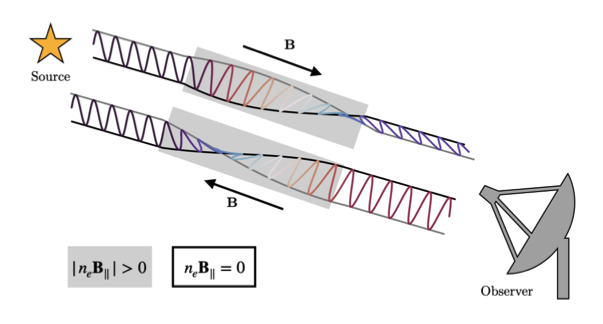
\includegraphics[width=0.8\linewidth]{Thesis_Template/Figures/Faraday_rot_diagram.png}
    \caption[Illustration of Faraday Rotation resulting from oppositely directed magnetic fields.]{A representation of Faraday Rotation as two electromagnetic waves travel from a source through two areas with oppositely orientated magnetic field (grey areas) towards the observer. The area with a magnetic field pointed towards the observer rotates the wave clockwise, whereas the area with a magnetic field pointed away from the observer rotates the wave anti-clockwise. Diagram from \cite{Emma_thesis}.}
    \label{fig:faraday rotation diagram}
\end{figure}

The FDF, $F(\phi)$ gives the intensity of polarised emission and polarisation angle as a function of FD and is defined by 

\begin{equation}
    P(\lambda^2) = \int_{\shortminus\infty}^{+\infty} F(\phi) e^{2i\phi\lambda^2}\space d\phi
    \label{eq: complex FDF}
\end{equation}

\noindent where $P(\lambda^2)$ is the complex fractional polarisation $P=\frac{Q+iU}{I}$. $Q+iU$ does not have a flat spectrum, so it will vary with frequency even in the absence of any Faraday rotation. Therefore $F(\phi)$ must also be a function of wavelength, $\lambda$. 

Equation \ref{eq: complex FDF} can be generalised using the weight function, also known as the sampling function, $W(\lambda^2)$ introduced in \cite{Brentjens_2005} to give the observed complex polarised emission:


\begin{equation}
    \Tilde{P}(\lambda^2) = W(\lambda^2)P(\lambda^2).
\end{equation}

\noindent The weight function is non zero at $\lambda^2$ where a measurement has been taken and zero elsewhere.

The Rotation Measure Spread Function (RMSF; $R(\phi)$) is another useful concept which is used to represent the beam within Faraday space and is defined as

\begin{equation}
    %R(\phi) = K \overset{m}{\underset{i=1}{\sum}}W(\lambda_i^2)e^{-2i\phi(\lambda_i^2-\lambda_0^2)}
    R(\phi) = e^{i(\phi\lambda_c^2)}\frac{sin(\phi\Delta\lambda^2)}{\phi\Delta\lambda^2},
    \label{eq: RMSF}
\end{equation}


\noindent where $\lambda_c$ is the central wavelength and $\Delta\lambda^2 = \lambda_2^2-\lambda_1^2$ is the width of $W(\lambda^2)$ (e.g. \cite{Dickey_2019}). The half power width of the RMSF represents the resolution in Faraday space and the sampling determines the sidelobe level. The FDF can also be deconvolved with the RMSF to remove the sidelobe response using the RMclean method described in \cite{Heald_2009}.

RM synthesis transforms the intensity and angle measured into Faraday depth space, with the discrete function described by the following equation from \cite{Brentjens_2005}:

\begin{equation}
    \Tilde{F}(\phi) \approx K \overset{m}{\underset{i=1}{\sum}}\Tilde{P}(\lambda_i^2)e^{\shortminus2i\phi(\lambda_i^2-\lambda_0^2)}    \label{eq: discrete rm synth}
\end{equation}

\noindent where $\Tilde{F}(\phi)$ is the reconstructed Faraday dispersion function. More details on this process can be found in Chapter \ref{ch: RMsynth}.

\subsection{Faraday Depolarisation}

Bandwidth depolarisation is an effect which occurs when Faraday rotation happens within an individual channel of bandwidth $\Delta\nu$ at wavelength $\lambda_0$ (with the corresponding frequency $\nu_0$) (e.g. \cite{Beck_cosmic}). When the Faraday rotation is averaged within this band when the measurement is taken, the true polarisation value can be distorted, resulting in depolarisation. This depolarisation can be described with the equation

\begin{equation}
    p = p_0 |\sin(\Delta\chi)/(\Delta\chi)|
    \label{eq: bandwidth depolarisation}
\end{equation}

\noindent where $p$ is the degree of synchrotron polarisation, $p_0$ is the intrinsic degree of linear polarisation and 
\begin{equation}
   \Delta\chi = 2\lambda_0^2{\rm{RM}}\Delta\nu/\nu_0.
   \label{eq: deltachi}
\end{equation}


\noindent \cite{Beck_cosmic} shows this places a limit on the maximum detectable RM of $RM_{max} \simeq \sqrt{3}/\Delta\nu$. 

Faraday depolarisation is caused by differential Faraday rotation. Differential Faraday rotation describes the effect of polarised planes of radio waves from the far side of the emitting layer being more rotated than those emitted from the near closest side, due to them passing through a magneto-ionic medium, or Faraday screen. The same effect can occur perpendicular to the line of sight, which can be indistinguishable from the first case if the FDF is the same. If the distribution of the emitting layer is assumed to have a symmetric magnetic field strength and distribution of thermal electrons along the line of sight, the degree of reduction of the polarisation can be described by a similar equation to Equation \ref{eq: bandwidth depolarisation} where it varies periodically with wavelength

\begin{equation}
    p = p_0 |\sin(2 RM \lambda^2)/(2RM\lambda^2)|
    \label{eq: Faraday depolarisation}
\end{equation}

\noindent and as it depends on RM, depolarisation therefore also depends on coherence length, field strength and thermal electron density. These periodic changes means that there is complete depolarisation at certain wavelengths. If the distribution is not perfectly symmetric, as is most often the case, non-periodic fluctuations in the polarisation occur as wavelength increases therefore complete depolarisation is very rare in reality.

There are thought to be two possible locations for the Faraday rotating medium in which the differential Faraday rotation takes place: internal, within the emission region itself, or external, within the foreground. To attempt to distinguish between the two requires high-resolution, low-frequency observations so that the Faraday screen is resolved, as extent of depolarisation has been shown to increase with decreasing frequency and resolution (e.g. \cite{cygnus_A}).

\subsection{Rotation Measure Grids}

With a large number of polarised background sources for which the RM has been determined, the Galactic magnetic field structure at varying scales can be probed by making a map, or grid, of these measurement (\cite{Johnston_2015}). These grids can be used to statistically probe extended foreground sources, such as the Milky Way and Magellanic Clouds (e.g. \cite{1980ApJ...242...74S}, \cite{1997A&A...322...98H}, \cite{Brown_2003}, \cite{Haverkorn_2006}), on $\sim$ kpc scale, galaxy clusters and the cosmic web on $\sim$ Mpc scales (e.g. \cite{Akahori_2014}) as well as supernova remnants, pulsars and bubbles within the Milky Way and other nearly galaxies on kpc-pc scales (e.g. \cite{1984ApJ...287..295M}, \cite{Gaensler_2001}). 

%Observations of large scale field patterns and their superpositions supports the dynamo theory whereas the lack of these patterns suggests this is not the case, and that the field maybe had a primordial origin or is structured by gas flows.

\begin{figure}
    \centering
    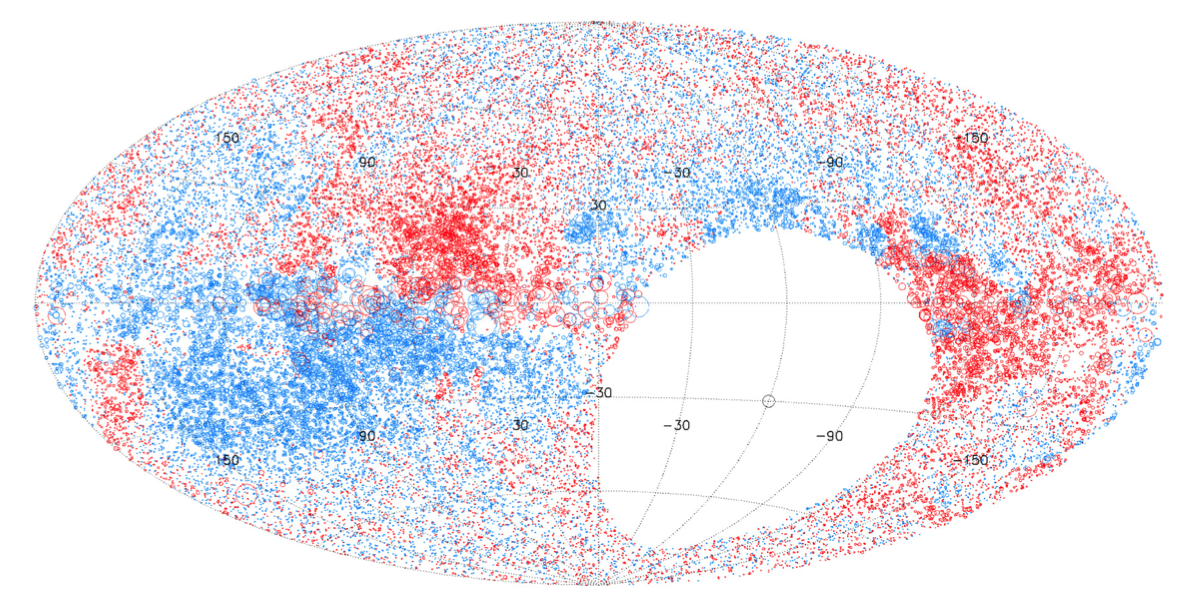
\includegraphics[width=\linewidth]{Thesis_Template/Figures/NVSS_RM_Grid.png}
    \caption[Rotation Measure grid showing sources from NVSS]{RM grid consisting of sources from NVSS, produced by \cite{Taylor_20009}, with red circles corresponding to positive rotation measure and blue to negative rotation measure and the size of the circle scales linearly with the magnitude of rotation measure.}
    \label{fig:Taylor RM grid}
\end{figure}

Large scale RM grids began to become a more widely used tool after \cite{Taylor_20009} re-analysed NRAO VLA Sky Survey (NVSS) data to calculate RM along the line of sight to 37,543 polarised sources (Figure \ref{fig:Taylor RM grid}). This grid has a resolution of $8^\circ$ and shows large scale structures which extend to high Galactic latitiudes. The RM grid has an average density on the sky of more than one RM per square degree, which was almost 2 orders of magnitude greater than any catalogue up to that point outside of the Galactic plane. Positive RM at each of the poles suggests that there is a sign reversal of the poloidal magnetic field across the Galactic plane. This catalogue has since been combined with other smaller RM catalogues by \cite{Oppermann_2012} which contains 41330 sources. \cite{Hutschenreuter_2020} then used a new inference algorithm to combine previous RM grids, using the table from \cite{van_eck_2022_6702843} to produce a profile of the Faraday sky, which is shown in Figure \ref{fig: Hutschenreuter 2020}.  This work was then updated to include almost all RM measurements available up to 2020 (\cite{Hutschenreuter_2022}). This catalogue 
consists of 55190 sources with a resolution of $1.3 
\times 10^{\shortminus2}$ square degrees. 
This resolution is twice that of previous endeavours. 
Much like the method used to produce the previous Hutschenreuter map, this map is produced using a Bayesian inference scheme. 

\begin{figure}
    \centering
    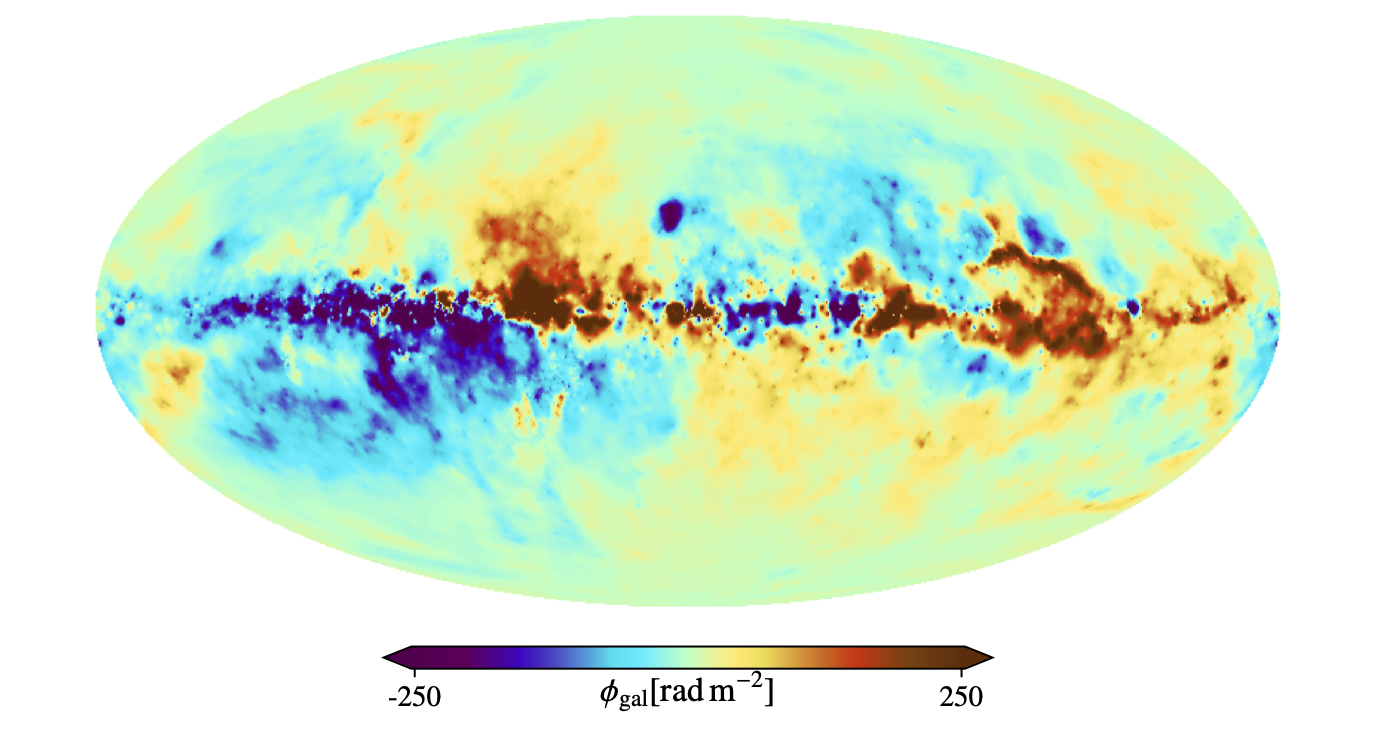
\includegraphics[width=\linewidth]{Thesis_Template/Figures/Hutschenreuter2020.png}
    \caption[Galactic Faraday Rotation measure distribution from \cite{Hutschenreuter_2020}]{The distribution of Galactic Faraday Rotation measure across the sky produced by \cite{Hutschenreuter_2020}, with the colour scale saturated at $\pm$ 250 rad$\,$m$^{\shortminus2}$}
    \label{fig: Hutschenreuter 2020}
\end{figure}

The most recent collection of RM has been compiled by \cite{vanEck_2023}. This catalogue was assembled to demonstrate the implementation of a proposed standard convention for RM catalogues, known as RMTable2023. This consolidates 55,819 RM from 42 published catalogues, making it the most comprehensive RM catalogue to date. These RM are shown Figure \ref{fig:van eck map}.

\begin{figure}
    \centering
    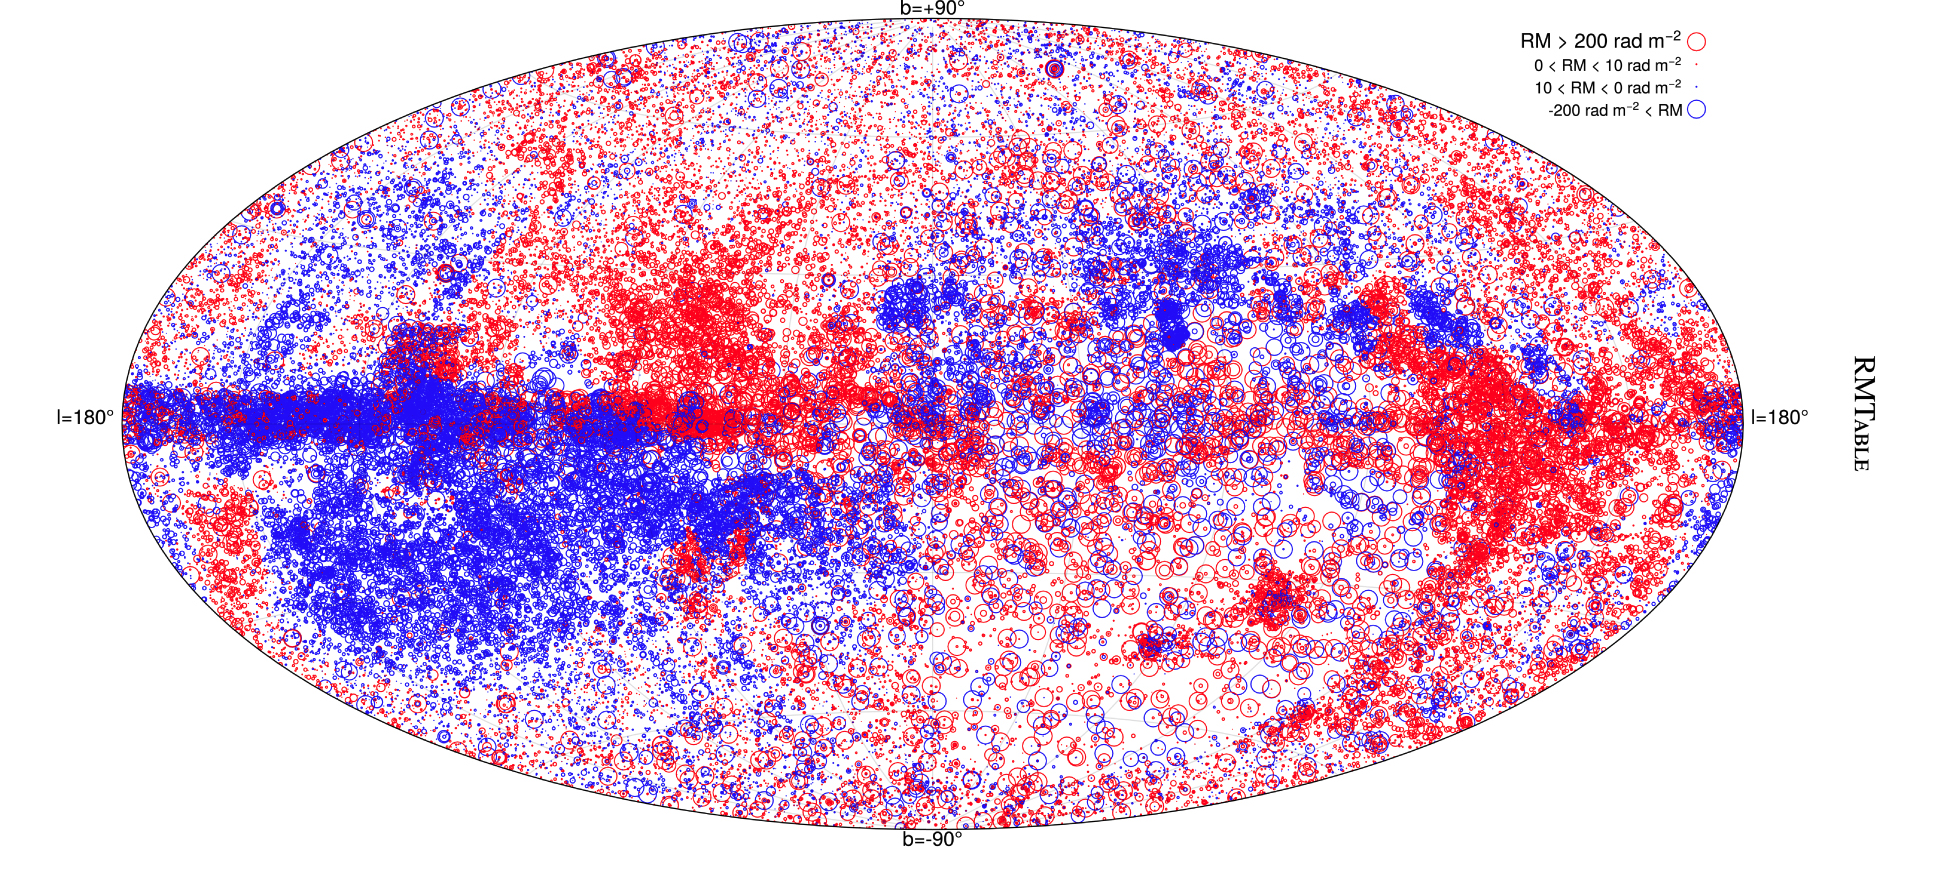
\includegraphics[width=\linewidth]{Thesis_Template/Figures/van eck map.png}
    \caption[Galactic Faraday Rotation measure distribution from \cite{vanEck_2023}]{Distribution of RM from \cite{vanEck_2023}. Each source is shown as a circle with diameter proportional to magnitude of RM, with the scale capped at 200 rad$\,$m$^{\shortminus2}$. Positive RMs are shown in red and negative in blue.}
    \label{fig:van eck map}
\end{figure}

These catalogues were lacking source density in the southern sky, however recent surveys such as S-PASS/ATCA (\cite{Schnitzeler_2019}) and the POlarised GLEAM Survey (POGS)
(\cite{POGS_2020}) have increased coverage in this region. 


Despite this progress, the average density over the entire sky is only 1.35 RM per square degree. This lack of density makes it difficult to detect and measure the small scale structure of the magnetic field. The southern hemisphere catalogues still have a much lower density than the NVSS region so the new all sky map does not have such an improved resolution as claimed. Ongoing projects such as SPICE-RACS (\cite{thomson2023rapidaskapcontinuumsurvey}) and POSSUM (\cite{POSSUM}) will further improve the southern density. 

Furthermore, it can be seen in Figure \ref{fig: Hutschenreuter 2020} that the structure appears to be more uniform at higher Galactic latitudes, and have a more complex structure along the Galactic plane. Higher resolution is needed to accurately map the rotation measure at low latitudes, as the average distance is much larger at low latitude so a higher density is required to accurately observed the structure in this region.  



\section{POSSUM}

The Polarization Sky Survey of the Universe's Magnetism (POSSUM)\footnote{https://possum-survey.org} is a commensal project using the Australian Square Kilometre Array Pathfinder (ASKAP) radio telescope as it observes for the EMU and WALLABY projects. This project will produce a continuum polarisation survey of the southern sky with a sensitivity of 17 $\mu$Jy/beam in Stokes Q and U and 30 $\mu$Jy/beam in Stokes I at 20" resolution with the aim to create a catalogue of Faraday rotation measures of various radio sources, including but not limited to radio galaxies, supernova remnants and pulsar wind nebulae (\cite{POSSUM}). When complete, the survey will have covered 20, 600 square degrees of the Southern sky.

ASKAP is a high dynamic range wide field survey telescope in a radio-quiet area of the Western Australia outback. Each of its 36 antennas has a 12-m diameter and is fitted with a focal plane phased-array feed (PAF) system which increases the field of view to 30 square degree (\cite{ASKAP}). A PAF consists of 188 receivers and low-noise amplifiers and is mounted at the focal point of each antenna. They are used to synthesise a 6 x 6 grid of virtual feeds which cover the field of view where each virtual feed has a primary beam defined by the telescope diffraction limit, $\theta = 1.22\frac{\lambda}{D}$. The telescope has a maximum baseline of $6\, {\rm km}$ and operates in the frequency range $0.7\shortminus1.8\, {\rm MHz}$.




Upon completion, POSSUM will have created an RM grid containing roughly one million linearly polarised sources. This grid will allow for study of the the magnetic field on smaller scales than previously possible due to its order-of-magnitude decrease in RM uncertainties, with a median uncertainty of $\approx 1$ rad$\,$m$^{\shortminus2}$. The completed RM grid will be about 30 times more dense than the data used for the most recently produced RM grid \cite{Hutschenreuter_2020}. POSSUM also measures RM in over 288 frequency channels, whereas NVSS only measured over 2 channels. This increase in frequency range allows for greater accuracy when the rotation between the channels is greater than 90$^\circ$, which is key for rapidly varying RM at low latitudes.

\subsection{Imaging Pipeline}


ASKAP-POSSUM pipeline, maintained and run by the ASKAP observatory, conducts calibration and imaging and produces the data products such as images and data cubes. Swiftly after each observation is complete it is processed by the pipeline. After initial flagging, the unpolarised calibrator source, which is PKS1934-638, is used to derive the bandpass, and then further flagging is applied to the target data after the bandpass solution is applied. Gain variations for each beam are then derived using a single amplitude and phase self calibration iteration. Images and Stokes spectral cubes are made and CLEANed independently per beam, Stokes parameter and channel \cite{Heald_2009}. The point spread functions (PSF) for each of the 36 beams are not identical due to sampling different spatial frequencies and different flagging so to combine the beams the smallest beam size for each channel is identified and then all beams are convolved to this beam size. The images from each beam are then linearly mosaicked, using full-Stokes models of the primary beam, to form a single image or data cube for that observation. The overlapping beams provide a near-uniform sensitivity across the field after this process. 

The standard image created has a 15 arcsecond resolution, but a high resolution image is also created which has a resolution of 9 arcseconds which gives four times as much detail as the standard image. This image is created reweighting the UV data with a uniform robustness, as opposed to the Briggs weighting used for the standard resolution image. The beam has a major and minor axis of 0.002 and a position angle of 77.05. Due to the new weighting, the high resolution image has almost twice the noise level as the standard image;  the high resolution image has a background noise level of $69\, \mu {\rm Jy}$ where as the standard image only has a noise level of $38 \, \mu {\rm Jy}$.

Finally, the source finding algorithm Selavy (\cite{Selavy_Whiting_2012}) is run on the standard Stokes I image to form a catalogue of sources, detailing their position and observed intensity. More details on this step are outlined in Section \ref{ch: sourcefinding}.

Another key part of this project is the science-ready processing pipeline, which contain the 1- and 3- dimensional polarimetry pipelines, which I have used to conduct the rotation measure synthesis. More information about these pipelines can be found in Sections \ref{POSSUM pipeline 1d} and \ref{3d pipeline}.

\subsection{Polarisation Leakage}

Polarisation leakage refers to the mixing of Stokes parameters observed by individual antennas of the interferometer, which means that the nominal polarisation recorded by each antenna distorts the true polarisation. This distortion can be quantified by a Mueller matrix (e.g. \cite{2009_mueller}, \cite{gil2022polarized}). Most noticeably, emission from Stokes I can appear to 'leak' into the other parameters, as it is the parameter with the highest intensity.  Leakage between Q and U is negligible in ASKAP (\cite{sault2015aces}) and is effectively independent of frequency.

During the imaging pipeline processing the UV data is corrected, using that assumption that the leakage is constant at the value measured from on-axis polarisation calibrators. This is referred to as the on-axis leakage correction. 

After the maps are made, the Q and U spectral cubes of each PAF beam are corrected for each component of the leakage that varies across the primary beam response in each PAF beam. This is referred to as the off-axis leakage correction. Leakage generally increases with distance from axis, so this is normally a larger correction than the on-axis correction. 

However, for early POSSUM observations, which were validated and accepted before 5th October 2023, which includes those in \cite{vanderwoude2024prototypefaradayrotationmeasure} and this dissertation, the off-axis correction actually included the leakage at the beam centre, which means that in effect the on-axis correction is applied twice. This creates an artificial leakage equal and opposite to the original on-axis leakage and resulted in an leakage of typically around $1\%$ of Stokes I into Stokes Q and U. The leakage does not vary greatly with frequency so produces a RM component close to 0 in the FDF. This has now been fixed and the leakage is mostly less than 0.05$\%$.

The on-axis instrumental polarisation calibration for each beam is derived once every 24 hours using the primary calibrator PKS B1934-638 and models of the ASKAP primary beams are found using holographic measurements of the unresolved, unpolarised calibrator source PKS B0408-65 (\cite{POSSUM}). Holographic techniques use a Fourier transform to find the aperture field distribution from the diffraction pattern. This distribution can then be used to characterise the surface of the antenna to give the axial offsets of individual structural panels (\cite{hotan2016holographic}).

\subsection{POSSUM Pilot}

POSSUM has had two pilot phases of 100 hours of observing time each. The first phase covered 270 square degrees and overlapped with the first EMU pilot survey but with a different, higher, frequency range. The second pilot phase was designed to test the efficacy of the projects commensality with EMU, in frequency band 1 (800$\shortminus$1088 MHz), and WALLABY, in frequency band 2 (1296$\shortminus$1440 MHz). The full survey is currently ongoing. 

\cite{vanderwoude2024prototypefaradayrotationmeasure} analysed four fields from the pilot observations, including one Galactic field in the ASKAP low band. The results from these four fields are the motivation for this work. The field that crossed the Galactic plane was found to have the lowest density of polarised sources of the fields investigated, with 20.2 RM per square degree, less than half that of the other fields that do not cross the Galactic plane. For this analysis, source finding was carried out by the ASKAP Observatory, who used the source finding software Selavy. Fewer sources were found in the Galactic field because Selavy works by finding islands above a threshold set by the local rms and in the plane this rms is set by the continuous band of Galactic nebulae rather than the expected thermal noise which is the case in the higher latitude fields. At low frequencies, below $\sim 100\,{\rm MHz}$, HII regions can be seen as discrete regions of absorption due to free-free absorption. This absorption leads to high opacity, depending on the line of sight between the observer and the HII region (\cite{free_free}). This problem of noise impacting the number of sources found is the key motivating factor for the work done for this dissertation.



The Galactic field has a line of sight through the Galactic plane, through the Scutum-Centaurus spiral arm of the Milky Way. It is noted that this field has much higher RM than the those in the other fields analysed in this paper, with a more complex structure.

\begin{figure}
    \centering
    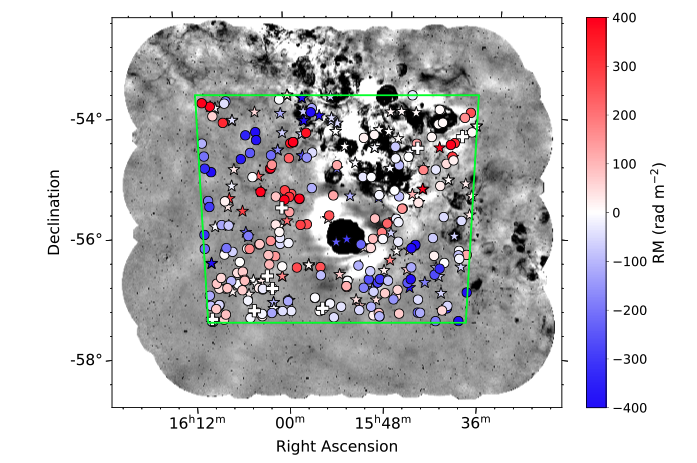
\includegraphics[width=0.9\linewidth]{Thesis_Template/Figures/Shannon_GL.png}
    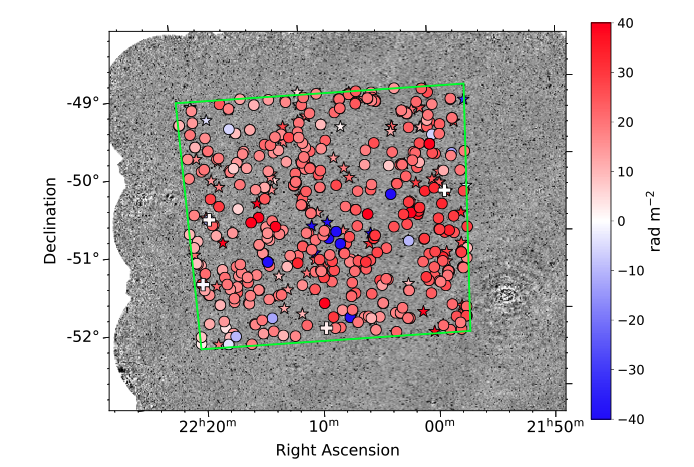
\includegraphics[width=0.9\linewidth]{Thesis_Template/Figures/Shannon_EC.png}
    \caption[Rotation measure grids form the POSSUM Pilot]{Rotation measure grids from the POSSUM Pilot, produced by \cite{vanderwoude2024prototypefaradayrotationmeasure} with positive RM pictured in red and negative RM pictured in blue. The upper plot shows a field at low Galactic latitude crossing the Galactic plane, where the RM values vary between $\pm$400 rad$\,$m$^{\shortminus2}$ and the lower plot shows a field at high Galactic latitude, where the RM varies between $\pm$ 40 rad$\,$m$^{\shortminus2}$}
    \label{fig: Shannon's RM grids}
\end{figure}

There are two key features of Figure \ref{fig: Shannon's RM grids} that have motivated my own project: firstly, that the density of sources significantly decreases within the diffuse emission of the Galactic plane, which limits the ability to probe the small scale structure of the Galactic magnetic field in this region. Secondly, it can be seen in the few RM we do have that there is significantly larger variation of the magnitude and sign of the RM on smaller scales, around 15 pc, within the diffuse emission of the Galactic plane. The range of RM in the Galactic plane field is approximately 10 times that of the field with a higher Galactic latitude. As discussed previously, understanding the smaller scale structure of our Galaxy is vital to determine the origins of the magnetic field itself. In order to better understand the rapidly varying nature of the small scale structure of the magnetic field along the Galactic plane, it is paramount that the source density within the diffuse emission is improved.



\section{Summary and Overview}

In this chapter I have given an outline of the relevant background science to this dissertation, such as a description of astrophysical and Galactic magnetic fields, methods for detecting them and the motivation for the work carried out for this dissertation. In Chapter \ref{ch: sourcefinding} I describe the method used to increase source density within the Galactic plane and information on the source finding algorithm used. In the next section, Chapter \ref{ch: RMsynth}, I explain the POSSUM analysis pipeline and how it was used to create a rotation measure grid of the field EMU1505-60. I also present the structure function analysis carried out on the RM grid. In Chapter \ref{ch: Canals} I detail the additional investigation I carried out to investigate the polarisation of diffuse emission, using 3D RM synthesis to produce RM and polarised intensity maps of the field and analysis canal like structure detected within RM maps of other POSSUM fields.

